\section{Имитация СХД}

Разработка СХД ведется в два этапа:
\begin{enumerate}
\item Разработка библиотеки, позволяющей создавать дискретно-событийные модели  
\item Реализация модели, имитирующей СХД Татлин.
\end{enumerate}

В главах \ref{LIB} и \ref{Tatlin} даётся описание каждой из этих частей, соответственно.

\section{Реализация дискретно-событийной библиотеки Simlibrary для моделирования СХД}\label{LIB}

\subsection{Введение}
В дискретно-событийно модели реализованы следующие сущности (рис. \ref{fig:libmodel}):
\begin{itemize}
\item Хост, с параметрами:
	\begin{itemize}
	\item Количество ядер
	\item Скорость (вычислительная мощность) во флопсах 	
	\end{itemize}
\item Сеть, с параметрами:
	\begin{itemize}
	\item 	Пропускная способность
	\item 	Задержка
	\end{itemize}
\item Диск, с параметрами:
	\begin{itemize}
	\item 	Размер накопителя
	\item 	Скорость на чтение 
	\item 	Скорость на запись
	\end{itemize}
\end{itemize}

\begin{figure}[!ht]
\centering
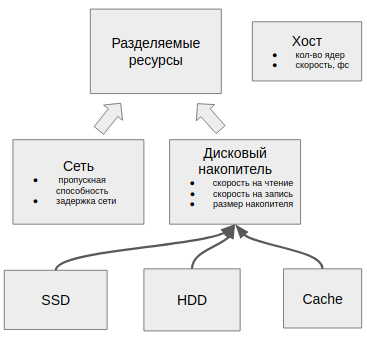
\includegraphics[width=10cm]{Kenenbek/images/libmodel.png}
\caption{Сущности, реализуемые в дискретно-событийной библиотеке}
\label{fig:libmodel}
\end{figure}

В файле $deployment.xml$ пользователь задаёт процессы, которые будут запущены в первый момент работы симуляции, например:

\begin{figure}[!ht]
\centering
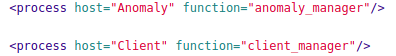
\includegraphics[width=10cm]{Kenenbek/images/deployfunc.png}
\caption{Пример стратегий-функций, которые будут запущены при старте симуляции}
\label{fig:deployfunc}
\end{figure}

Рис. ~\ref{fig:deployfunc} говорит о том, что при старте симуляции будут запущены две процесса, которые будут имитировать какой-либо реальный процесс при помощи функций $anomaly\_manager$ и $client\_manager$ соответственно. 

\par 
Каждый из запущенных процессов создаёт события (также могут создаваться другие процессы), которые добавляются в глобальную очередь событий. Существует процесс-мастер, который занимается поиском события из очереди, которое должно реализоваться в текущий момент (таким событием выбирается объект с минимальным временем окончания). Время окончания текущего события является текущим временем симуляции. После этого подсчитывается количество времени, прошедшее с прошлого события и обновляется очередь. Схематично данный процесс показан на рис. \ref{fig:libstep}.
 
\begin{figure}[!ht]
\centering
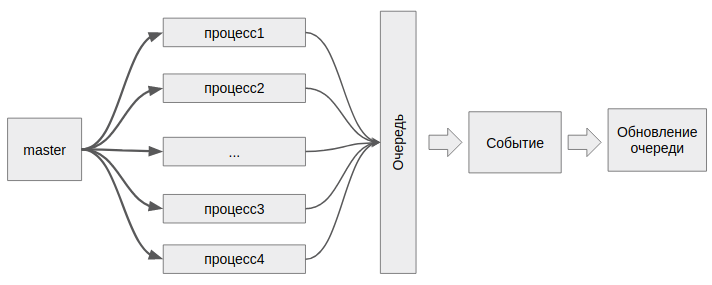
\includegraphics[width=\textwidth]{Kenenbek/images/libstep.png}
\caption{Один шаг работы симуляции}
\label{fig:libstep}
\end{figure}

\subsection{Особенности языка Go}
\par
Go (часто также Golang) — компилируемый многопоточный язык программирования. Он разрабатывался как язык программирования для создания высокоэффективных программ, работающих на современных распределённых системах и многоядерных процессорах. Среди его особенностей можно отметить:

\begin{itemize}
\item Простой и понятный синтаксис.
\item Статическая типизация. Позволяет избежать ошибок, допущенных по невнимательности, упрощает чтение и понимание кода, делает код однозначным.
\item Скорость и компиляция. Скорость у Go в десятки раз быстрее, чем у скриптовых языков, при меньшем потреблении памяти. При этом, компиляция практически мгновенна. Весь проект компилируется в один бинарный файл, без зависимостей. Как говорится, «просто добавь воды». И вам не надо заботиться о памяти, есть сборщик мусора.
\item Отход от ООП. В языке нет классов, но есть структуры данных с методами. Наследование заменяется механизмом встраивания. Существуют интерфейсы, которые не нужно явно имплементировать, а лишь достаточно реализовать методы интерфейса.
\item Параллелизм. Параллельные вычисления в языке делаются просто, изящно и без головной боли. Горутины (что-то типа потоков) легковесны, потребляют мало памяти.
\item Богатая стандартная библиотека. В языке есть все необходимое для веб-разработки и не только. Количество сторонних библиотек постоянно растет. Кроме того, есть возможность использовать библиотеки C и C++.
\item Возможность писать в функциональном стиле. В языке есть замыкания (closures) и анонимные функции. Функции являются объектами первого порядка, их можно передавать в качестве аргументов и использовать в качестве типов данных.
\end{itemize}

\subsubsection{Типы данных в Go}

\paragraph{Числа.}
В Go существуют следующие типы целых чисел: uint8, uint16, uint32, uint64, int8, int16, int32 и int64. 8, 16, 32 и 64 говорит нам, сколько бит использует каждый тип. uint означает «unsigned integer» (беззнаковое целое), в то время как int означает «signed integer» (знаковое целое). Беззнаковое целое может принимать только положительные значения (или ноль). В дополнение к этому существуют два типа-псевдонима: byte (то же самое, что uint8) и rune (то же самое, что int32).
\par 
В Go есть два вещественных типа: float32 и float64 (соответственно, часто называемые вещественными числами с одинарной и двойной точностью).
\paragraph{Строки.} 
Cтрока (string) — это последовательность символов определенной длины, используемая для представления текста. Строки в Go состоят из независимых байтов, обычно по одному на каждый символ.
\paragraph{Массив.} 
Массив — это нумерованная последовательность элементов одного типа с фиксированной длиной. В Go они выглядят так (рис. \ref{fig:go-slice}):

\begin{figure}[!ht]
\centering
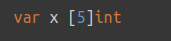
\includegraphics[width=3cm]{Kenenbek/images/go-slice.png}
\caption{Инициализация списка в Go}
\label{fig:go-slice}
\end{figure}

x — это пример массива, состоящего из пяти элементов типа int
\paragraph{Словарь.} 
Словарь (также известен как ассоциативный массив или карта) — это неупорядоченная коллекция пар вида ключ-значение. Карта представляется в связке с ключевым словом $map$, следующим за ним типом ключа в скобках и типом значения после скобок. Читается это следующим образом: «x — это карта string-ов для int-ов». Пример на рис. \ref{fig:go-map}

\begin{figure}[!ht]
\centering
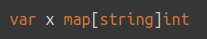
\includegraphics[width=3cm]{Kenenbek/images/go-map.png}
\caption{Инициализация словаря в Go}
\label{fig:go-map}
\end{figure}

\paragraph{Указатели.} Указатель (pointer) — переменная, диапазон значений которой состоит из адресов ячеек памяти или специального значения — нулевого адреса. Оно используется для указания того, что в данный момент указатель не ссылается ни на одну из допустимых ячеек. В Go указатели представлены через оператор $\*$ (звёздочка), за которым следует тип хранимого значения. $\*$ также используется для «разыменовывания» указателей. Также существует оператор $\&$, который используется для получения адреса переменной.

\subsubsection{Как задаются функции в Go}
\par
Функция является независимой частью кода, связывающей один или несколько входных параметров с одним или несколькими выходными параметрами. 
Функция начинается с ключевого слова func, за которым следует имя функции. Аргументы (входы) определяются так: имя тип, имя тип, $\ldots$. За параметром следует возвращаемый тип. В совокупности аргументы и возвращаемое значение также известны как сигнатура функции. Далее идет тело функции, заключенное в фигурные скобки. 
Функции (также известные как процедуры и подпрограммы) можно представить в виде схемы, как показано на рисунке \ref{fig:func}.

\begin{figure}[!ht]
\centering
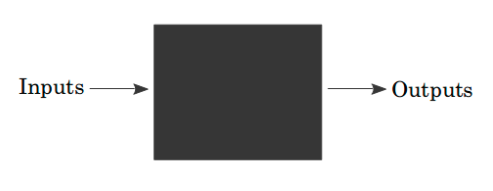
\includegraphics[width=10cm]{Kenenbek/images/func.png}
\caption{Схематическое представление функции}
\label{fig:func}
\end{figure}

В общем виде синтаксис функций представляется в виде (рис. \ref{fig:func-body}):

\begin{figure}[!ht]
\centering
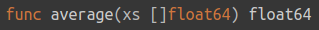
\includegraphics[width=5cm]{Kenenbek/images/func-body.png}
\caption{Заголовок функции, где average представляеи имя функции, xs []float64 -- список чисел типа float64, за скобками указывается тип возращаемого значения.}
\label{fig:func-body}
\end{figure}

\par 
В функции имеется также оператор возврата, который немедленно прервет выполнение функции и вернет значение, указанное после оператора, в функцию, которая вызвала текущую.


\subsection{Описание окружения имитации}

Имитация системы происходит при помощи объекта типа Environment, который полностью отражает текущее положение системы. Данный объект обладает следующими полями:

\textbf{currentTime}
Текущее время системы типа $float64$. Изменяется дискретными шагами.

\textbf{workers}
Словарь типа $map[uint64]*Process$, где в качестве ключа выступает идентификатор PID объекта, а в качестве значение указатель $Worker$.

\textbf{routesMap}  
Словарь типа  $map[Route]*Link$. Содержит значения обо всех путях, возможной в данной конфигурации компьютерной сети. $Route$ -- структура, имеющая в качестве своих полей $start$ и $finish$ -- указатели на хост, которые являются началом и концом пути, соответственно. Значение $*Link$ -- является указателем на сеть, по которой будет проходить передача пакетов в обе стороны.


\textbf{queue}
Поле типа $eventQueue$. Является глобавльным хранилищем всех событий во время имитации сложных сложных систем.

\textbf{mutex}         
Поле типа $sync.Mutex$. Примитив синхронизации нужный для того, чтобы обеспечивать консистентность доступа к данным, таким как очередь событий $queue$. 

\textbf{shouldStop}    
Поле типа $bool$. Во время прогона симуляции является равным 1. После того, как все события в имитации заканчиваются, либо при наличии специального события, выставляется в отрицательное значение и прогон прекращается.

\textbf{hostsMap}      
Словарь типа $map[string]HostInterface$. Содержит информацию обо всех хостах, которые имеются в симуляции. В качестве ключа словаря -- имя хоста, в качестве значения интерфейс типа HostInterface, который обобщает такие типы как $host$, $NetworkSwitch$ и $IOBalancer$.

\textbf{vesninServers}
Поле типа $[]*Host$. Является списком, который содержит информацию о рабочих дисковых контроллерах, поддреживающих отношения с клиентом, представленных в виде указателя на $*Host$.

\textbf{allVesninServers}
Поле типа $[]*Host$. Поле типа $[]*Host$. Является списком, который содержит информацию о обо всех (рабочих и нерабочих) дисковых контроллерах, поддреживающих отношения с клиентом, представленных в виде указателя на $*Host$.

\textbf{storagesMap}   
Словарь типа $map[string]*Storage$. В данном контейнере хранится информация обо всех дисках, примонтированных к системе хранения данных. В качестве ключа словаря используется идентификатор конечного хранилища данных, а качестве значения -- указатель на дисковое хранилище.

\textbf{linksMap}      
Словарь типа $map[string]*Link$. Контейнер, содержащий информацию обо всех сетях, представленных в данной симуляции.  В качестве ключа словаря используется идентификатор сети, а качестве значения -- сеть, по которой будет идти передача данных.

\textbf{FunctionsMap} 
Словарь типа $map[string]func(*Process, []string)$. Данный контейнер хранит информацию обо всех фукнциях, которые будует запущены в качестве горутин в начальный момент времени (время запуска симуляции). Функции должны быть объявлены в файле deployment.xml.  В качестве ключа словаря используется идентификатор функции, представленный в строковом виде, а качестве значения -- указатель на функцию.

\textbf{daemonList}  
Поле типа $[]*Process$. Является списком, который содержит информацию о горутинах, которые во время симуляции СХД, являются представлениями Unix-демонов и самостоятельно должны завершить своё исполнение.

\textbf{pid} 
Поле типа $ProcessID$. Указатель на функцию, которая исполняется в текущий момент времени.

\textbf{waitWorkerAmount} 
Поле типа $uint64$. Количество горутин, запущенных в текущий момент времени, завершения которых нужно ожидать для того, чтобы наполнить очередь актуальными текущими событиями. 

\textbf{stepEnd}        
Поле типа $chan interface{}$. Является средством коммукации горутин с главной ($master$) горутиной. В данный канал связи горутины, которые исполняются в текущий момент времени, сигнализируют о своём завершении.

\textbf{nextWorkers}
Поле типа $[]*Process$. Является списком, который содержит информацию о горутинах, которые должны буть запущены на следующем шаге работы имитации системы со статусом $OK$.

\textbf{timeOutWorkers}   
Поле типа $[]*Process$. Является списком, который содержит информацию о горутинах, которые должны буть запущены на следующем шаге работы имитации системы со статусом $TIMEOUT$.

\textbf{anomalyWorkers}   
Поле типа $[]*Process$. Является списком, который содержит информацию о горутинах, которые должны буть запущены на следующем шаге работы имитации системы со статусом $FAIL$.

\textbf{logsMap}  
Словарь типа $map[string]float64$. Данный контейнер хранит информацию, которая впоследствии будет выведена в виде логов системы.  В качестве ключа словаря используется идентификатор наблюдаемого значения, а качестве значения -- числовая характеристика данной величины.

\textbf{unitsMap} 
Словарь типа $map[string]float64$. Данный контейнер хранит информацию о единицах системы измерений, принятых в данной симуляции. В качестве ключа словаря используется идентификатор единицы измерения, а качестве значения -- численная характерстика относительно эталона.

\textbf{backupRoutesMap} 
Словарь типа  $map[Route]*Link$. Содержит значения обо всех запасных (backup) путях, возможной в данной конфигурации компьютерной сети. $Route$ -- структура, имеющая в качестве своих полей $start$ и $finish$ -- указатели на хост, которые являются началом и концом пути, соответственно. Значение $*Link$ -- является указателем на сеть, по которой будет проходить передача пакетов в обе стороны.

\textbf{HostLinksMap}
Словарь типа $map[HostInterface][]*Link$. Данный контейнер хранит информацию о сетях, к которым имеет доступ каждый хост. В качестве ключа словаря используется идентификатор хоста, а качестве значения -- список, состоящий из указателей на сеть, принадлежащих даннному хосту.

\textbf{LinkBackupsMap}  
Словарь типа $map[*Link]*Link$.  В качестве ключа словаря используется идентификатор конечного хранилища данных, а качестве значения -- указатель на дисковое хранилище.

\subsubsection{Функции Environment}
\par 
Дискретно-событийная симуляция моделирует работу системы как дискретную последовательность событий во времени. Каждое событие происходит в определенный момент времени и отмечает изменение состояния в системе. Между последовательными событиями никаких изменений в системе не предполагается; таким образом, симуляция может непосредственно переходить во времени от одного события к другому. Схема данного действия изображена на рис. ~\ref{fig:loop}.
\par 
Это отличает данную модель с непрерывной по времени симуляцией, в которой симуляция непрерывно отслеживает динамику системы с течением времени. Вместо того, чтобы быть основанным на событиях, данная модель называется симуляцией на основе действий (activity-based); время разбивается на небольшие срезы времени, а состояние системы обновляется в соответствии с набором действий, происходящих во временном фрагменте. Поскольку симуляции дискретных событий не должны имитировать каждый временной срез, они обычно могут выполняться намного быстрее, чем соответствующая непрерывная по времени симуляция.
\par 
Однако существует еще и является трехфазный подход к моделированию дискретных событий (планируется сделать в будущем). В этом подходе первая фаза (этап) -- переход к следующему хронологическому событию. Второй этап -- выполнить все события, которые безоговорочно (unconditionally) произойдут в это время (они называются B-событиями). Третья фаза - это выполнение всех событий, которые условно происходят в это время (они называются C-событиями). Трехфазный подход -- это усовершенствование подхода, основанного на событиях, в котором упорядочены одновременные события, чтобы максимально эффективно использовать компьютерные ресурсы. Данный подход предлагается использовать в будущем.

\begin{figure}[!ht]
\centering
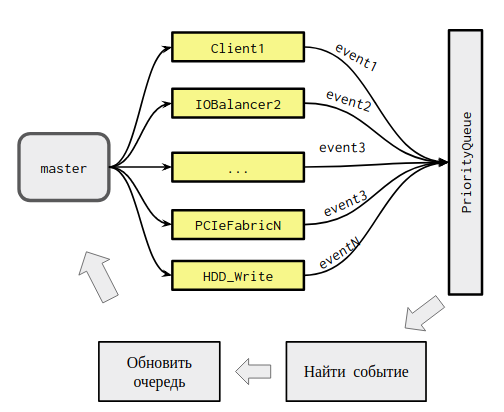
\includegraphics[width=\textwidth]{Kenenbek/images/loop.png}
\caption{Один цикл симуляции}
\label{fig:loop}
\end{figure}  

\textbf{func NewEnvironment() *Environment}

Входные аргументы: отсутсвуют.

Выходное значение: переменнная типа *Environment.

Описание функции:Создаёт и инициализует необходимые поля для функцирования симуляции, такие как:
\begin{itemize}
\item 		queue           
\item 		workers        
\item 		SendEventsNameMap 
\item 		ReceiveEventsNameMap
\item 		ReceiverSendersMap
\item 		stepEnd
\item 		logsMap
\item 		HostLinksMap
\item 		LinkBackupsMap
\end{itemize}

\textbf{func createUnits()}

Входные аргументы: отсутствуют.

Выходное значение: отсутствует.

Описание функции: Инциализирует единицы измерения необходимые при симуляции системы (показано в таблице ~\ref{tab:SI}\ref{tab:SI}{tab:SI}).
\begin{table}[]
\centering
\caption{Единицы системы измерений при моделировании}
\label{tab:SI}
\begin{tabularx}{\textwidth}{|X|X|}
TB   & $1000^4$ byte         \\
GB   & $1000^3$              \\
MB   & $1000^2$              \\
KB   & $1000$                \\
B    & $1$                   \\
GBps & $1000^3$ byte per sec \\
MBps & $1000^2$ byte per sec \\
KBps & $1000$ byte per sec   \\
Bps  & $1$ byte per sec      \\
Gf   & $1000^3$ flops        \\
Mf   & $1000^2$ flops        \\
Kf   & $1000$ flops          \\
f    & $1$ flops            
\end{tabularx}
\end{table}

\textbf{func (env *Environment) stopSimulation(EventInterface)}

Входные аргументы: указатель на объект типа *Environment.

Выходное значение: отсутствует.

Описание: Даннная функция останавливает исполнение программы путем выставления флага shouldStop в положительное значение.

\textbf{func (env *Environment) updateQueue(deltaTime float64) }

Входные аргументы: указатель на объект типа *Environment.

Выходное значение: отсутствует.

Описание: Даннная функция обновляет очередь событий за время $deltaTime$. 

\textbf{func (env *Environment) CreateTransferEvents()}

Входные аргументы: указатель на объект типа *Environment.

Выходное значение: отсутствует.

Описание: Даннная функция создаёт события, которые имитируют передачу данных от одного хоста к другому.

\textbf{func (env *Environment) Step() EventInterface }

Входные аргументы: указатель на объект типа *Environment.

Выходное значение: текущее событие симуляции.

Описание: Даннная функция осуществляет шаг симуляции, который состоит из следующих шагов. 
\begin{enumerate}
\item Cоздать события, которые имитируют передачу данных от одного хоста к другому.
\item Проверить является ли этот шаг симуляции последним.
\item Проверить симуляцию на возникновение дедлоков.
\item Получить событие из очереди с минимальным значением времени.
\item Обновить текущее время.
\item Обновить очередь событий за время, прошедшее с времени прошлого события.
\item Обработать коллбэки (callbaks) текущего события.
\item Проверить является ли этот шаг симуляции последним.

\end{enumerate}

\textbf{func (env *Environment) FindNextWorkers(event EventInterface)}

Входные аргументы: указатель на объект типа *Environment, текущее событие EventInterface.

Выходное значение: отсутствует. 

Описание: Даннная функция занимается поиском горутин, которые должны начать исполнение после выполнения текущего шага. Данный список включает в себе также горутины, которые начнут исполнение со статусами $OK$, $FAIL$, $TIMEOUT$.

\textbf{func (env *Environment) SendStartToSignalWorkers()}

Входные аргументы: указатель на объект типа *Environment.

Выходное значение: отсутствует. 

Описание: Даннная функция рассылает сигналы через каналы коммуикации горутинам, которые должны начать исполнение после выполнения текущего шага. Данный список включает в себе также горутины, которые начнут исполнение со статусами $OK$, $FAIL$, $TIMEOUT$.

\textbf{func (env *Environment) WaitWorkers() }

Входные аргументы: указатель на объект типа *Environment.

Выходное значение: отсутствует. 

Описание: Даннная функция дожидается выполнения задач текущими горутинами, которым были посланы сигналы на предыдущем этапе.



\subsection{Описание примитивов, использованных при имитации системы}

\subsubsection{Имитация сети}
\par 
Компьютерная сеть или сеть передачи данных - это цифровая телекоммуникационная сеть, которая позволяет узлам совместно использовать ресурсы. В компьютерных сетях вычислительные устройства обмениваются данными друг с другом с использованием соединений между узлами (линией передачи данных). Эти линии передачи данных устанавливаются на кабельных носителях, таких как провода или оптические кабели.
Сетевые компьютерные устройства, которые создают, маршрутизируют и завершают данные, называются сетевыми узлами. Узлы могут включать хосты, такие как персональные компьютеры, телефоны, серверы, а также сетевое оборудование. Можно сказать, что два таких устройства объединены в сеть, когда одно устройство может обмениваться информацией с другим устройством, независимо от того, имеет ли оно прямое соединение друг с другом. В большинстве случаев протоколы связи конкретного приложения являются многоуровневыми (то есть переносятся как полезная нагрузка) по другим более общим протоколам связи.

Сеть имитируется при помощи структуры $Link$. Она обладает следующими полями (характеристиками). 

\textbf{name}
Идентификатор сети в текстовом представлении типа string. 

\textbf{state}	 float64
Степень соответсвия изначальному ресурсу, либо 1 минус деградация данной сети. Значение типа float64, может принимать значения от 0 до 1, где 0 соответсвует полной деградации сети, а 1 -- "фабричному" состоянию. 

\textbf{route}	 *Route
Указатель на структуру данных Route, которая содержит информацию о хостах, которые соединяет данная сеть. 

\textbf{minEvent}	
Указатель на минимальное событие-пакет *TransferEvent, которое передаётся в текущий момент по сети. 

\textbf{bandwidth}	 
Переменная типа float64. Пропускная способность сети, которая изменяется в байтах в секунду. 

\textbf{lastTimeRequest}
Переменная типа float64. Время последнего обращения к данной сети.

\textbf{mutex}	           
Примитив синхронизации типа sync.Mutex необходимой для корректности парального доступа к полям структуры данной сети.
 
\textbf{counter}
Переменная типа int64. Количество пакетов, которые передаются в текущий момент времени по сети. 


\textbf{func NewLink(bandwidth float64, name string) *Link}

Входные аргументы: bandwidth -- переменная типа float64. Содержит информацию о пропускной способности сети. name -- переменная типа string, имя сети. 

Выходное значение: Указатель созданную структуру, которая инкапсулирует сеть. 

Описание функции: Создаёт указатель созданную структуру, которая инкапсулирует сеть с именем name и пропускной способностью bandwidth и инициализирует необходимые поля сети, такие как:

\begin{itemize}
\item bandwidth 
\item mutex    
\item name   
\item state  
\end{itemize}




\textbf{func (link *Link) Put(e *TransferEvent)}

Входные аргументы: Указатель на структуру *Link, указатель на событие, которое должно передаваться по сети.

Выходное значение: отсутствует.

Описание функции: Данная функция добавляет событие в очередь событий, относящейся к сети link. 


\textbf{func (link *Link) EstimateTimeEnd(e *SendEvent)}

Входные аргументы: Указатель на структуру Link; указатель на событие SendEvent, которое должно передаваться по сети.

Выходное значение: отсутствует

Описание функции: Оценить время окончания  $t_{end}$ передачи события-пакета по данной сети по следующей формуле:

\[ t_{end} = t_0 + \dfrac{S}{\dfrac{B}{n}  \cdot q }  \], 

где $t_0$ -- это текущее время, \(S\) -- размер передаваемого пакета,  \(B\) -- пропускная способность сети, \(n\) -- количество пакетов, которые передаются в текущий момент времени,  \(q\) -- степень деградации сети. 


\textbf{func (env *Environment) FindNextTransferEvent()}

Входные аргументы: Указатель на структуру *Environment.

Выходное значение: Отсутствует. 

Описание функции: Данная функция "составляет" события, которые будут передаваться в текущий момент времени.  


\textbf{func GetRoute(route Route) *Link}

Входные аргументы: route переменна типа Route, содержащая информацию об начальном и конечном хостах.

Выходное значение: Указатель на структуру Link. 

Описание функции: Данная функция по имени route возвращает указатель на структуру Link.


\textbf{Route} обладает следующими полями.

Указатель на начальный	start. Тип  HostInterface

Указатель на конечный finish. Тип HostInterface

\subsubsection{Имитация хоста}

\par 
Сетевой хост - это компьютер или другое устройство, подключенное к компьютерной сети. Сетевой хост может предоставлять информационные ресурсы, службы и приложения пользователям или другим узлам в сети. Сетевой узел - это сетевой узел, которому назначен сетевой адрес.
Компьютеры, участвующие в сетях, которые используют пакет интернет-протокола, также могут называться IP-узлами. В частности, компьютеры, участвующие в Интернете, называются интернет-хостами, иногда интернет-узлами. Интернет-хосты и другие IP-хосты имеют один или несколько IP-адресов, назначенных их сетевым интерфейсам. Адреса настраиваются либо вручную администратором, либо автоматически. В общем случае, все серверы - это хосты, но не все хосты - это серверы. Любое устройство, установившее соединение с сетью, квалифицируется как хост, тогда как только хосты, которые принимают подключения от других устройств (клиентов), квалифицируются как серверы.

\textbf{name}      
Поле типа string. Является идентификатором объекта.  

\textbf{typeId} 
Поле типа string. Содержит информацию о классе устройств, которым принадлежит данный хост. 

\textbf{processes} 
Поле типа []*Process. Содержит информацию в виде списка указателей на Process обо всех текущих процессах, запущенных на данном хосте. 

\textbf{speed}     
Поле типа float64. Скорость работу данного хоста, измеряемая в flops.

\textbf{storage}   
Поле типа *Storage. Содержит указатель на диск, который примонтирован к данному хосту.

\textbf{traffic} 
Поле типа float64. Траффик в байт/с, который проходит через данный хост.

\textbf{logs} 
Поле типа interface\{\}. Текстовове представление логов данного хоста.

\textbf{Функции необходимые для имитации хоста}

\textbf{func (env *Environment) getHostByName(name string) HostInterface}

Входные аргументы: Аргумент name типа string.

Выходное значение: Объект типа HostInterface.

Описание функции: Данная функция по данному имени name возвращает объект типа HostInterface.


\textbf{func (process *Process) GetHost() HostInterface }

Входные аргументы: Указатель на процесс, владеющий в данное время исполнением.

Выходное значение: Объект типа HostInterface

Описание функции: Данная функция возвращает хост HostInterface, на котором в данное время исполняется текуща горутина. 

\textbf{func (host *Host) GetName() string }

Входные аргументы: Указатель на объект Host.

Выходное значение: Идентификатор хоста тип string.

Описание функции: Данная функция возвращает имя текущего хоста.


\textbf{func (host *Host) GetType() string }

Входные аргументы: Указатель на объект Host.

Выходное значение: Тип класса устройств к которым относится данный хост. Текстовое представление.

Описание функции: Данная функция возвращает тип текущего хоста.


\textbf{func (host *Host) GetDevTemp() float64 }

Входные аргументы: Указатель на объект Host.

Выходное значение: Температура данного хоста. Тип float64.

Описание функции: Данная функция возвращает температуру данного хоста в текущий момент времени.


\textbf{func (host *Host) GetTraffic() float64}

Входные аргументы: Указатель на объект Host.

Выходное значение: Суммарный (входной и выходной) траффик, проходящий, через данный хост. 

Описание функции: Данная функция возвращает значение суммарного (входного и выходного) траффика, проходящего, через данный хост.


\textbf{func (host *Host) AddTraffic(traffic float64)}

Входные аргументы: Указатель на объект Host.

Выходное значение: Отсутствует.

Описание функции: Данная функция кумулятивно увеличивает суммарное значение выходного траффика на значение traffic. 


\textbf{func (host *Host) GetLoad() int }

Входные аргументы: Указатель на объект Host.

Выходное значение: Загрузка процессора в текущий момент времени.

Описание функции: Данная функция возвращает загрузку процессора в текущий момент времени.


\textbf{func (host *Host) GetLogs() interface}

Входные аргументы: Указатель на объект Host.

Выходное значение: Логи компоненты системы. 

Описание функции: Данная функция возвращает логи компоненты системы. 


\textbf{func (host *Host) SetLogs(logs interface)}

Входные аргументы: Указатель на объект Host.

Выходное значение: Отсутствует.

Описание функции: Обновляет логи текущей компоненты системы. 


\textbf{func (host *Host) GetStorage() *Storage }

Входные аргументы: Указатель на объект Host.

Выходное значение: Указатель на объект Storage, объект симулирующий конечный дисковый носитель.

Описание функции: Данная функция возвращает указатель на объект Storage, объект симулирующий конечный дисковый носитель.


\textbf{func GetHostByName(hostName string) HostInterface }

Входные аргументы: Строка -- имя запрашиваемого хоста. 

Выходное значение: Указатель на объект Host.

Описание функции: Данная функция возвращает указатель на объект Host по его строковому указателю.

\subsubsection{Имитация конечного дискового хранилища}
\textbf{StorageType}
Структура данных StorageType необходима при модировании класса конечных дисковых носителей. Данная структура обладает следующими полями:

\textbf{	typeId}. Тип    string. Идентификатор класса, к которому принадлежит данный тип конечных дисковых носителей. 
\textbf{	writeRate}. Тип float64. Скорость данных на запись конечного дискового носителя.
\textbf{	readRate }. Тип float64. Скорость данных на чтение конечного дискового носителя.
\textbf{	size     }. Тип float64. Размер конечного дискового носителя.

Конкретная реализация конечного дискового носителя осуществляеся при помощи примитива Storage. Он обладает следующими полями. 

\textbf{	*StorageType}. Указатель на класс устройств конечного дискового носителя. 
\textbf{	name     }. Тип string. Идентификатор конечного дискового носителя.
\textbf{	readLink }. Тип *Link. Указатель структуру, по которой происходит запись на  конечный дисковый носитель.
\textbf{	writeLink }. Тип *Link. Указатель структуру, по которой происходит чтение на  конечный дисковый носитель.

\textbf{	usedSize }. Тип int64. Занятое место на конечном дисковом носителе.
\textbf{	logs }. Тип interface{}. Логи, принадлежащие конечному дисковому носителю.


\textbf{func NewStorage(storageType *StorageType, name string) *Storage}

Входные аргументы: Тип конечного носителя storageType, имя, создаваемого объекта, name. 

Выходное значение: Указатель на объект Storage. 

Описание функции: Данная функция создаёт объект, имитирующий поведение конечного диского носителя.

\textbf{func GetDiskDrives() map[string]*Storage}

Входные аргументы: отсутствуют.

Выходное значение: Словарь, где в качестве ключа используется строка, а качестве значения конечный дисковый носитель, имеющий такое же имя.

Описание функции: Данная функция возвращет словарь, содержащий сведения обо всех дисковых носителях, имеющихся в конкретной реализации. 

\textbf{func (storage *Storage) GetLogs() interface{}}

Входные аргументы: Указатель на структуру, имитирующую конечный дисковый накопитель.

Выходное значение: Логи дискового компонента. 

Описание функции: Данная функция возвращает логи дисковой компоненты. 

\textbf{func (storage *Storage) SetLogs(logs interface{})}

Входные аргументы: Указатель на структуру, имитирующую конечный дисковый накопитель.

Выходное значение:  Отсутствует.

Описание функции: Данная функция обновляет логи дисковой компоненты. 

\textbf{func (storage *Storage) GetName() string}

Входные аргументы: Указатель на структуру, имитирующую конечный дисковый накопитель.

Выходное значение: Имя конечного дискового накопителя.

Описание функции: Данная функция имя конечного дискового накопителя.

\textbf{func (storage *Storage) GetDevTemp() float64}

Входные аргументы: Указатель на структуру, имитирующую конечный дисковый накопитель.

Выходное значение: Температура конечного дискового накопителя.

Описание функции: Данная функция возвращает температуру конечного дискового накопителя.

\textbf{func (storage *Storage) GetRawCapacity() float64}

Входные аргументы: Указатель на структуру, имитирующую конечный дисковый накопитель.

Выходное значение: Заявленная ёмкость конечного дискового накопителя.

Описание функции: Данная функция возвращает ёмкость конечного дискового накопителя.

\textbf{func (storage *Storage) GetAvgReadSpeed() float64}

Входные аргументы: Указатель на структуру, имитирующую конечный дисковый накопитель.

Выходное значение: Средняя скорость на чтение конечного дискового накопителя.

Описание функции: Данная функция возвращает средную скорость на чтение конечного дискового накопителя.

\textbf{func (storage *Storage) GetAvgWriteSpeed() float64}

Входные аргументы: Указатель на структуру, имитирующую конечный дисковый накопитель.

Выходное значение: Средняя скорость на запись конечного дискового накопителя.

Описание функции: Данная функция возвращает средную скорость на запись конечного дискового накопителя.
 

\textbf{func (storage *Storage) GetDataInterfaceCNT() uint16}

Входные аргументы: Указатель на структуру, имитирующую конечный дисковый накопитель.

Выходное значение: Интерфейс передачи данных. 

Описание функции: Данная функция возвращает интерфейс передачи данных.

\textbf{func (storage *Storage) GetUsedSpace() float64 }

Входные аргументы: Указатель на структуру, имитирующую конечный дисковый накопитель.

Выходное значение:  Размер занятого места на конечном дисковом накопителе.

Описание функции: Данная функция возвращает размер занятого места на конечном дисковом накопителе.

\textbf{func (storage *Storage) GetFreeSpace() float64}

Входные аргументы: Указатель на структуру, имитирующую конечный дисковый накопитель.

Выходное значение: Размер свободного места на конечном дисковом накопителе.

Описание функции: Данная функция возвращает размер свободного места на конечном дисковом накопителе.

\textbf{func (storage *Storage) WritePacketSize() }

Входные аргументы: Указатель на структуру, имитирующую конечный дисковый накопитель.

Выходное значение: Отсутствует.

Описание функции: Данная функция имитирует запись на конечный дисковый накопитель одного пакета данных.

\textbf{func (storage *Storage) DeletePacketSize()}

Входные аргументы: Указатель на структуру, имитирующую конечный дисковый накопитель.

Выходное значение: Отсутствует.

Описание функции: Данная функция имитирует удаление с конечного дискового накопителя одного пакета данных.

\subsubsection{Имитация типов хранения информации}
В системах хранения данных существует три типа хранения данных:
\begin{enumerate}
\item Блочный тип 
\item Файловая система 
\item Объектный тип
\end{enumerate}

\par
Блочный тип хранения данных использует "сырое" устройство и работает с битами и байтами, в то время как файлая система и объектное хранилище работают на более абстрактном уровне, и, как следует из названия, работают с файлами и папками.  
\par
Блок, иногда называемый физической записью, представляет собой последовательность байтов или бит, обычно содержащую некоторое количество записей, имеющих максимальную длину, размер блока. Данные имеющие такую структуру называются блочными. 	Процесс помещения данных в блоки на конечном хранилище информации называется блокингом, а деблокинг - процессом извлечения данных из блоков. Блокинг данные обычно хранятся в буфере данных и одновременно считывают или записывают целый блок. Блокинг снижает накладные расходы и ускоряет обработку потока данных. Для некоторых устройств, таких как магнитная лента и дисковые устройства, блокинг уменьшает объем внешнего хранилища, необходимого для данных. Блочный тип хранения данных практически повсеместно используется при хранении данных на 9-дорожечной магнитной ленте, флэш-памяти NAND и вращающихся носителях, таких как гибкие диски, жесткие диски и оптические диски.
\par 
Большинство файловых систем основаны на блочном типе хранения данных, которое является уровнем абстракции для аппаратного обеспечения, ответственного за хранение и извлечение определенных блоков данных, хотя размер блока в файловых системах может быть кратным размеру физического блока. Это приводит к неэффективности пространства из-за внутренней фрагментации, поскольку длины файлов часто не являются целыми кратными размеру блока, и, таким образом, последний блок файла может оставаться частично пустым. Это создаёт свободное пространство, которое тяжело использовать. Некоторые новые файловые системы, такие как Btrfs и FreeBSD UFS2, пытаются решить эту проблему с помощью методов, называемых блочным субаллокацией и слиянием хвостов. Другие файловые системы, такие как ZFS, поддерживают переменные размеры блоков.
\par 
Блочный уровень при хранении данных обычно абстрагируется файловой системой или системой управления базами данных (СУБД) для использования приложениями и конечными пользователями. Физические или логические тома, к которым обращаются через блок ввода-вывода, могут быть устройствами, внутренними для сервера, напрямую подключенными через SCSI или Fibre Channel, или удаленными устройствами, доступными через сеть хранения данных (SAN) с использованием протокола, такого как iSCSI или AoE. DBMS часто используют свой собственный блок ввода-вывода для повышения производительности и возможности восстановления по сравнению с разбиением базы данных поверх файловой системы.
\par 
Файловая система контролирует, как данные сохраняются и извлекаются. Без файловой системы информация, размещенная на носителе данных, будет представлять собой один большой объем данных без возможности указать, где останавливается одна часть информации и начинается следующая. Разделяя данные на куски и давая каждой части имя, информация легко изолируется и идентифицируется. Принимая свое название от того, как названы информационные системы на бумажной основе, каждая группа данных называется «файлом». Структура и логические правила, используемые для управления группами информации и их именами, называются «файловой системой».
\par 
Существует много разных типов файловых систем. Каждый из них имеет разную структуру и логику, свойства скорости, гибкости, безопасности, размера и т. д. Например, на графике \ref{fig:fsystem} изображена иерархия взаимодействия компонентов компьютерной системы. Некоторые файловые системы были разработаны для использования в конкретных приложениях. К примеру, файловая система ISO 9660 разработана специально для оптических дисков. 

\begin{figure}[!ht]
\centering
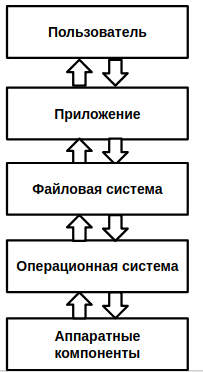
\includegraphics[width=5cm]{Kenenbek/images/fsystem.png}
\caption{Иерархия взаимодействия компонент компьютерной системы}
\label{fig:fsystem}
\end{figure}

\par
Файловые системы могут использоваться на различных устройствах различного типа, которые используют различные типы носителей. Сегодня самым распространенным устройством хранения данных является жесткий диск. Другие типы носителей, которые используются, включают флэш-память, магнитные ленты и оптические диски. В некоторых случаях, например, с tmpfs, основная память компьютера (оперативное запоминающее устройство, ОЗУ) используется для создания временной файловой системы для краткосрочного использования.
\par 
Некоторые файловые системы используются на локальных устройствах хранения данных, другие предоставляют доступ к файлам через сетевой протокол (например, NFS, SMB или 9P-клиенты). Некоторые файловые системы являются «виртуальными», что означает, что предоставленные «файлы» (называемые виртуальными файлами) вычисляются по запросу (например, procfs и sysfs) или представляют собой просто сопоставление с другой файловой системой, используемой в качестве хранилища резервных копий. Файловая система управляет доступом как к содержимому файлов, так и к метаданным об этих файлах. Он отвечает за организацию пространства для хранения; надежность, эффективность и настройка в отношении физического носителя данных являются важными конструктивными соображениями.

\par 

Объектное хранилище (также известное как объектно-ориентированное хранилище) представляет собой архитектуру хранения компьютерных данных, которая манипулирует данными как объектами, в отличие от других архитектур хранения, таких как файловые системы, которые управляют данными как иерархии файлов, и блочной памяти, которая управляет данными как блоки в секторах и дорожках. Каждый объект обычно включает в себя сами данные, переменное количество метаданных и глобально уникальный идентификатор. Хранилище объектов может быть реализовано на нескольких уровнях, включая уровень устройства (устройство хранения объектов), уровень системы и уровень интерфейса. В каждом случае хранилище объектов пытается включить возможности, не разрешенные другими архитектурами хранения, такими как интерфейсы, которые могут быть непосредственно программируемыми приложением, пространство имен, которое может охватывать несколько экземпляров физического оборудования, и функции управления данными, такие как репликация данных и распределение данных при детализации детализации.

\par 
Томом или логическим диском является единая доступная область хранения с одной файловой системой, обычно (хотя и не обязательно), находящаяся на одном разделе жесткого диска. Хотя логический диск может отличаться от физического диска, его можно получить с помощью логического интерфейса операционной системы. Однако, следует иметь ввиду, что логический диск отличается от раздела. Например, это иллюстрирует следующая таблица ~\ref{tab:volumetable}.


\begin{table}[]
\centering
\caption{Пример разбиения физического диска на логические диски}
\label{tab:volumetable}
\begin{tabularx}{\textwidth}{|l|l|l|l|}
\hline
Физический диск & Раздел   & Файловая система & Наименование \\ \hline
Жесткий диск №1 & Раздел 1 & NTFS             & С:           \\ \hline
Жесткий диск №1 & Раздел 2 & FAT32            & D:           \\ \hline
Жесткий диск №2 & Раздел 1 & FAT32            & E:           \\ \hline
\end{tabularx}
\end{table}

\par 
Рассмотрим случай организации логического диска путем объединения нескольких конечных дисковых носителей. При такой организации получается возможной параллельная запись/чтение на диск путём использования нескольких головок. На рис. ~\ref{fig:volume} показана схема параллельной записи на диск. 
\begin{figure}[!ht]
\centering
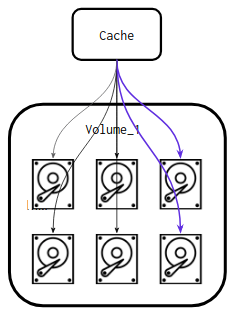
\includegraphics[width=5cm]{Kenenbek/images/volume.png}
\caption{Пример записи на логический диск. Черная линия демонстрирует запись оригинальных данных, синияя -- parity кодов}
\label{fig:volume}
\end{figure}


\subsubsection{Имитация коммутатора внутренней управляющей сети СХД}
\textbf{NetworkSwitch}
Структура данных NetworkSwitch необходима при моделировании коммутатора внутренней управляющей сети СХД. Данная структура обладает следующими функциями:

\textbf{func(ns *NetworkSwitch) GetConnectedDevCnt() uint8}

Входные аргументы: Указатель на структуру, имитирующую коммутатор внутренней управляющей сети СХД.

Выходное значение: Количество подключенных устройств.

Описание функции: Данная функция возвращает количество подключенных устройств.

\textbf{func(ns *NetworkSwitch) GetOnlineSwitchesCnt() uint8}

Входные аргументы: Указатель на структуру, имитирующую коммутатор внутренней управляющей сети СХД.

Выходное значение: Количество одновременно включенных коммутаторов.

Описание функции: Данная функция возвращает количество одновременно включенных коммутаторов.

\subsubsection{Имитация фабрики PCI Express}
\textbf{PCIeFabric}
Структура данных PCIeFabric необходима при моделировании фабрики PCI Express. Данная структура обладает следующими функциями:

\textbf{func(pc *PCIeFabric) GetPCIeDevicesCnt() uint16}

Входные аргументы: Указатель на структуру, имитирующую фабрику PCI Express.

Выходное значение: Количество подключенных устройств.

Описание функции: Данная функция возвращает количество подключенных устройств.


\textbf{func(pc *PCIeFabric) GetPCIeMaxBandw() float64}

Входные аргументы: Указатель на структуру, имитирующую фабрику PCI Express.

Выходное значение: Максимальная пропускная способность.

Описание функции: Данная функция возвращает значение максимальной пропускной способности.

\subsubsection{Имитация балансировщика нагрузки}
\textbf{IOBalancer}
Структура данных IOBalancer необходима при моделировании балансировщика нагрузки. Данная структура обладает следующими полями:

\textbf{	*Host}. Наследование от базового типа Host, т.е помимо нижеперечисленных полей, тип IOBalancer обладает также и полями типа Host. 
\textbf{	readResponseTime}. Тип float64. Время отклика на запросы чтения.
\textbf{	writeResponseTime}. Тип float64. Время отклика на запросы записи.
\textbf{	writeRequests}. Тип float64. Количество запросов на запись в единицу времени.
\textbf{	readRequests}. Тип  float64. Количество запросов на чтение в единицу времени.
\textbf{	lastTime}. Тип float64. Время последнего запроса. 


\textbf{func(iob *IOBalancer) GetReadRequestsRate() float64}

Входные аргументы: Указатель на структуру, имитирующую балансировщик нагрузки.

Выходное значение: Количество обработанных запросов на чтение в секунду.

Описание функции: Данная функция возвращает количество обработанных запросов на чтение в секунду.

\textbf{func(iob *IOBalancer) GetWriteRequestsRate() float64}

Входные аргументы: Указатель на структуру, имитирующую балансировщик нагрузки.

Выходное значение: Количество обработанных запросов на запись в секунду. 

Описание функции: Данная функция возвращает количество обработанных запросов на запись в секунду.

\textbf{func(iob *IOBalancer) GetReadResponseDelay() float64}

Входные аргументы: Указатель на структуру, имитирующую балансировщик нагрузки.

Выходное значение: Время отклика при запросе на чтение. 

Описание функции: Данная функция возвращает значение времени отклика при запросе на чтение.

\textbf{func(iob *IOBalancer) GetWriteResponseDelay() float64}

Входные аргументы: Указатель на структуру, имитирующую балансировщик нагрузки.

Выходное значение: Время отклика при запросе на запись.

Описание функции: Данная функция возвращает значение временпи отклика при запросе на запись.

\textbf{func(iob *IOBalancer) GetReadDataVolume() float64}

Входные аргументы: Указатель на структуру, имитирующую балансировщик нагрузки.

Выходное значение: Объем передаваемых данных в режиме на чтение.

Описание функции: Данная функция возвращает объем передаваемых данных в режиме на чтение.

\textbf{func(iob *IOBalancer) GetWriteDataVolume() float64}

Входные аргументы: Указатель на структуру, имитирующую балансировщик нагрузки.

Выходное значение: Объем передаваемых данных в режиме на запись. 

Описание функции: Данная функция возвращает объем передаваемых данных в режиме на запись.

\textbf{func(iob *IOBalancer) GetReadRequestProcessTime() float64}

Входные аргументы: Указатель на структуру, имитирующую балансировщик нагрузки.

Выходное значение: Среднее время обработки запросов на чтение.

Описание функции: Данная функция возвращает среднее значение времени обработки запросов на чтение.

\textbf{func(iob *IOBalancer) GetWriteRequestProcessTime() float64}

Входные аргументы: Указатель на структуру, имитирующую балансировщик нагрузки.

Выходное значение: Среднее время обработки запросов на запись.

Описание функции: Данная функция возвращает возвращает среднее значение времени обработки запросов на запись.

\textbf{func(iob *IOBalancer) GetIoProcessingMethod() uint8}

Входные аргументы: Указатель на структуру, имитирующую балансировщик нагрузки.

Выходное значение: Способ обработки операций ввода-вывода (синхронный/асинхронный).

Описание функции: Данная функция возвращает способ обработки операций ввода-вывода (синхронный/асинхронный).

\textbf{func(iob *IOBalancer) GetReadCancelRate() float64}

Входные аргументы: Указатель на структуру, имитирующую балансировщик нагрузки.

Выходное значение: Количество аннулированных запросов на чтение в единицу времени.

Описание функции: Данная функция возвращает количество аннулированных запросов на чтение в единицу времени.

\textbf{func(iob *IOBalancer) GetWriteCancelRate() float64}

Входные аргументы: Указатель на структуру, имитирующую балансировщик нагрузки.

Выходное значение: Количество аннулированных запросов на запись в единицу времени. 

Описание функции: Данная функция возвращает количество аннулированных запросов на запись в единицу времени.

\textbf{func(iob *IOBalancer) GetBlockSize() uint16}

Входные аргументы: Указатель на структуру, имитирующую балансировщик нагрузки.

Выходное значение:  Размер блока данных при чтении/записи.

Описание функции: Данная функция возвращает  размер блока данных при чтении/записи.

\textbf{func(iob *IOBalancer) GetIOProcessCnt() uint8}

Входные аргументы: Указатель на структуру, имитирующую балансировщик нагрузки.

Выходное значение: Количество процессов, генерирующих запросы на чтение/запись.

Описание функции: Данная функция возвращает количество процессов, генерирующих запросы на чтение/запись.

\textbf{func(iob *IOBalancer) GetReadQueueLength() uint8}

Входные аргументы: Указатель на структуру, имитирующую балансировщик нагрузки.

Выходное значение: Длина очереди запросов на чтение для асинхронных операций ввода-вывода.

Описание функции: Данная функция возвращает длину очереди запросов на чтение для асинхронных операций ввода-вывода.

\textbf{func(iob *IOBalancer) GetWriteQueueLength() uint8}

Входные аргументы: Указатель на структуру, имитирующую балансировщик нагрузки.

Выходное значение: Длина очереди запросов на запись для асинхронных операций ввода-вывода. 

Описание функции: Данная функция возвращает длину очереди запросов на запись для асинхронных операций ввода-вывода.

\textbf{func(iob *IOBalancer) SetReadResponseDelay(rt float64}

Входные аргументы: Указатель на структуру, имитирующую балансировщик нагрузки; время отклика запросов на чтение rt.

Выходное значение: Отсутствует 

Описание функции: Данная функция устанавливает время отклика при запросах на чтение.

\textbf{func(iob *IOBalancer) SetWriteResponseDelay(rt float64}

Входные аргументы: Указатель на структуру, имитирующую балансировщик нагрузки; время отклика запросов на запись rt.

Выходное значение: Отсутствует.

Описание функции: Данная функция устанавливает время отклика при запросах на чтение.

\subsubsection{Имитация задач в симуляторе}
\textbf{Task}
Структура данных Task необходима при моделировании задач в симуляторе. Данная структура обладает следующими полями, характеризующими  её:

\textbf{	name}. Тип  string. Идентификатор задачи.

\textbf{	size}. Тип float64. Размер задачи в байтах. Необходим в случае передачи данных по сети или сохранении задачи на диск.

\textbf{	flops}. Тип   float64. Вычислительная сложность задачи во флопсах. Необходима для оценки времени, которое затратит хост при обработке данной задачи.

\textbf{	data}. Тип interface{}. Ссылка на дополнительную структуру данных, которыми может обладать данная задача. 

Соответственно, данный тип данных обладает следующим набором функций:

\textbf{func NewTask(name string, flops float64, size float64, data interface{}) *Task}

Входные аргументы: имя задачи, вычислительный размер задачи, размер задачи, ссылка на дополнительную структуру данных.

Выходное значение: Объект типа Task.

Описание функции: Данная функция создаёт задачу с параметрами, указанными во входных аргументах.

\textbf{	func (task *Task) GetName() string }

Входные аргументы: Отсутствуют.

Выходное значение: Идентификатор задачи. 

Описание функции: Данная функция возвращает идентификатор задачи.

\textbf{	func (task *Task) GetSize() float64 }

Входные аргументы: Отсутствуют.

Выходное значение: Размер задачи.

Описание функции: Данная функция возвращает размер задачи.

\textbf{	func (task *Task) GetFlops() float64}

Входные аргументы: Отсутствуют.

Выходное значение: Вычислительный размер задачи.

Описание функции: Данная функция возвращает вычислительный размер задачи.

\textbf{	func (task *Task) GetData() interface{} }

Входные аргументы: Отсутствуют.

Выходное значение: Ссылка на дополнительную структуру данных, которыми может обладать данная задача.

Описание функции: Данная функция возвращает ссылка на дополнительную структуру данных, которыми может обладать данная задача.

\textbf{	func (process *Process) Execute(task *Task) }

Входные аргументы: Задача, которую необходимо обработать.

Выходное значение: Статус выполения задачи.

Описание функции: Данная функция имитирует поведение СХД при исполнении задачи.


Структура Process обладает следующими методами.

\textbf{func (pid *ProcessID) Next() uint64}

Входные аргументы: Указатель на структуру, которая симулирует процесс.

Выходное значение: Идентификатор объекта.

Описание функции: Данная функция генерирует новый уникальный идентификатор для процесса.

\textbf{func ProcWrapper(processStrategy func(*Process, []string), w *Process, args []string)}

Входные аргументы: Указатель на структуру, которая симулирует процесс, указатель на функцию, которая будет симулировать стратегию, которая реализовавается на реальном хосте, набор аргументов, которым обладает хост.

Выходное значение: Процесс.

Описание функции: Данная функция по указанным входным параметрам создаёт и запускает процесс.


\textbf{func (process *Process) Daemonize() }

Входные аргументы: Указатель на структуру, которая симулирует процесс.

Выходное значение: Отсутствует.

Описание функции: Данная функция превращает текущий процесс в процесс-демон.


\textbf{func (p *Process) GetData() interface}

Входные аргументы: Указатель на структуру, которая симулирует процесс.

Выходное значение: Указатель на структуру данных о дополнительных параметрах, которыми обладает хост.

Описание функции: Данная функция возвращает указатель на струку данных о дополнительных параметрах, которыми обладает хост.


\textbf{func (p *Process) GetName() string}

Входные аргументы: Указатель на структуру, которая симулирует процесс.

Выходное значение: Имя процесса.

Описание функции: Данная функция имя процесса.

\textbf{func (p *Process) GetEnv() *Environment}

Входные аргументы: Указатель на структуру, которая симулирует процесс.

Выходное значение: Объект, указывающий на окружение имитации.

Описание функции: Данная функция возвращает объект, указывающий на окружение имитации.

\subsubsection{Имитация процессов}
\par 
Процесс представляет собой экземпляр выполнения какой-либо логики последовательности действий в симуляции. Он содержит программный код и его текущую деятельность.


\textbf{Process}
Структура данных Process необходима при моделировании процессов в симуляторе. Данная структура обладает следующими полями, характеризующими  её:

\textbf{	pid}. Тип uint64. Идетификатор процесса. 

\textbf{	env}. Тип        *Environment. Ссылка на Environment, в котором осуществляется симуляция. 

\textbf{	resumeChan}. Тип chan STATUS. Канал по которому осуществляется взаимодействие главной горутины с данной горутиной. 

\textbf{	host}. Тип       HostInterface. Хост на котором существует данный процесс. 

\textbf{	name}. Тип         string. Имя данного процесса. 

\textbf{	noMoreEvents}. Тип bool. Булева переменная, которая выставляется в положительное значение, при завершение работы процесса.

\textbf{	data}. Тип         interface. Ссылка на  структуру, в  которой может содержаться дополнительная информация о данном процессе.

\textbf{	Done}. Тип chan struct. Канал по которому данный процесс сообщает мастерской горутине о своём завершении. 

\subsection{Устройство очереди}

Наиболее важным элементом при реализации моделирования сложных систем является поддержание консистентности очереди событий. В текущей версии библиотеки она реализована при помощи встроенного в язык программирования интерфейса "container/heap". Данный интерфейс представляет структуру данных под названием дерево, которое обладает свойством, что каждая его узел является минимальным значением в его поддереве. Эта структура данных была выбрана для моделирования, т.к является наиболее распространенной при реализации очереди событий с приоритетом, которым в случае моделирования событийных имитаций является время окончания события. 

Для имплементации данного интерфейса были реализованы следующие функции, которые показаны в таблице \ref{tab:queue}. 

\begin{table}[]
\centering
\caption{Функции необходимые для реализации на очереди}
\label{tab:queue}
\begin{tabularx}{\textwidth}{|X|X|X|X|}
\hline
Функция                                      & Входные аргументы                                                          & Выходные аргументы                              & Описание функции                                                                                                                                                                                                         \\ \hline
func (eq eventQueue) Len() int               & -                                                                          & Длина очереди, тип int                          & Данная функция возвращает значение длины очереди.                                                                                                                                                                        \\ \hline
func (eq eventQueue) Less(i, j int) bool     & Индексы элементов очереди. Тип int                                         & Тип bool                                        & Данная функция задаёт правило сравнения и  сравнивает элемент очереди с индексом i c элементом с индексом j. В случае, если первый элемент больше, то возвращается логическое да, в противном случает -- логическое нет. \\ \hline
func (eq eventQueue) Swap(i, j int)          & Индексы элементов очереди. Тип int                                         & -                                               & Данная функция меняет местами элемент очереди с индексом i c элементов очереди с идексом j.                                                                                                                              \\ \hline
func (eq *eventQueue) Push(e interface\{\})  & Значение, которое необходимо добавить в очередь. Тип interface\{\}         & -                                               & Данная функция добавляет новый элемент e в очередь событий.                                                                                                                                                              \\ \hline
func (eq *eventQueue) Pop() interface\{\}    & -                                                                          & Минимальнй элемент в очереди. Тип interface\{\} & Данная функция извлекает минимальный элемент из очереди событий.                                                                                                                                                         \\ \hline
func(eq *eventQueue) Fix(h Interface, i int) & h - элемент в очереди, который нуждается в изменениях. i - новый приоритет & -                                               & Данная функция меняет приоритет у элемента h в очереди событий на приоритет i.                                                                                                                                           \\ \hline
\end{tabularx}
\end{table}

\subsection{Имитация аномалий}

Компоненты компьютерной системы, т.е устройства, предназначенное для автоматического выполнения последовательных действий в соответствии с заложенной стратегией, можно сгруппировать по три основные категории:
\begin{itemize}
\item Хост. Данный тип устройств нужен для моделирования следующих сущностей, т.е его обязанности входит имитация получения, отправления, и обработки информации. При имитации СХД Татлин  хостами также являются:
	\begin{itemize}
		\item Сервер
		\item Коммутатор внутренней сети управления
		\item PCIe фабрика 
	\end{itemize}
\item Сеть (кабель)
\item Хранилище данных (HDD, SSD, кэш)
\end{itemize}
Исходя из вышеперечисленного списка можно выделить три типа аномалий:
\begin{itemize}
\item Аномалии хостов
\item Аномалии дисков
\item Аномалии хранилищ данных
\end{itemize}
 В текущей версии реализации дискретно-событийной модели имплементировано два вида аномалий: хостов и сетей. Реализация аномалий для конечных хранилищ намечена на ближайшее будущее/второй квартал.

\subsubsection{Аномалия сети}

Аномалия сети моделируется при помощи следующей последовательности действий:

\begin{enumerate}
\item Выставить пропускную способность, трафик через данную сеть равными нулю. (bandwidth = 0)
\item Найти все пакеты, передаваемые по этим сетям. (task, queue)
\item Удалить пакеты из глобальной очереди событий. (task, queue)
\item Уведомить процессы, которые принимали/передавали пакеты об статусом передачи $FAIL$. (task, queue, status, process)
\end{enumerate}

Реализация этой парадигмы показана на рис. ~\ref{fig:anom-link}.

\begin{figure}[!ht]
\centering
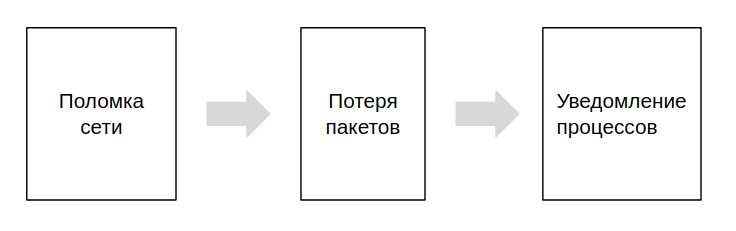
\includegraphics[width=10cm]{Kenenbek/images/anom-scheme-link.png}
\caption{Аномалия сети}
\label{fig:anom-link}
\end{figure}

\subsubsection{Аномалия хоста}

Аномалия хоста моделируется при помощи следующей последовательности действий:

\begin{enumerate}
\item Выставить вычислительную мощность хоста равной нулю. (host)
\item Найти все исходящие/входящие кабели из/в данный хост. (host, link)
\item Выставить пропусные способности (степень деградации), трафик через данные сети равными нулю. (bandwidth, state, traffic)
\item Найти все пакеты, передаваемые по этим сетям. (task)
\item Удалить их из глобальной очереди событий. (task, queue)
\item Уведомить процессы, которые принимали/передавали пакеты об статусом передачи $FAIL$. (process, status)
\item Прекратить выполнение задач, исполняемых на данном хосте, со статусом $FAIL$. (process, status)

\end{enumerate}

Реализация этой парадигмы показана на рисунке ~\ref{fig:anom-host}.

\begin{figure}[!ht]
\centering
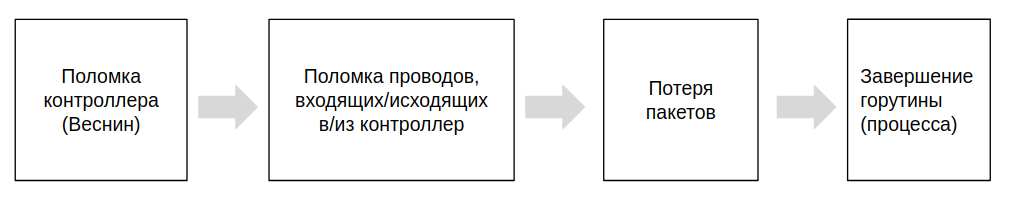
\includegraphics[width=10cm]{Kenenbek/images/anom-scheme-host.png}
\caption{Аномалия хоста}
\label{fig:anom-host}
\end{figure}

Восстановление хоста моделируется как показано на рис. ~\ref{fig:repai-host} при следующей последовательности действий:

\begin{enumerate}
\item Выставить степень деградации данного хоста равной нулю (state)
\item Найти все исходящие/входящие провода из/в данный хост. (host, link)
\item Выставить степень деградации данных сетей равной нулю. (link, bandwidth)
\end{enumerate}

\begin{figure}[!ht]
\centering
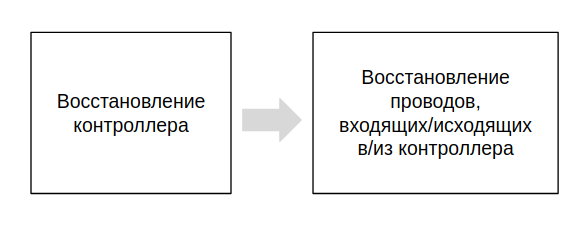
\includegraphics[width=10cm]{Kenenbek/images/repair-host.png}
\caption{Восстановление хоста}
\label{fig:repai-host}
\end{figure}

\subsection{Перечень функций, импортированных при симуляции СХД Татлин}.

Все нижеперечисленные функции обладают указателем на процесс, от лица которого имитируется действие.

При симулировании приёма/передачи файла существует три кода возврата:
\begin{itemize}
\item OK --- сообщение об успешной передаче файла
\item FAIL --- сообщение о неуспешной передаче файла, т.к возникла поломка компоненты, участвующей при передача файла
\item TIMEOUT --- сообщение о неуспешной передаче файла, т.к действие не было завершено в течение отведенного промежутка времени
\end{itemize}  

\textbf{func (worker *Process) SendTask(task *Task, address string) STATUS}

Входные аргументы: Указатель на передаемую задачу; адрес по которому процесс отправляет  задачу

Возвращаемое значение: Статус об успешной отправке файла

Описание функции: Данная функция имитирует отправку файла по заданному адресу. Данная функция является блокирующей. 

\textbf{func (worker *Process) SendTaskWithTimeout(task *Task, address string, timeout float64) STATUS}

Входные аргументы:Указатель на передаемую задачу;адрес по которому процесс отправляет  задачу, время ожидание отправки файла

Возвращаемое значение: Статус об отправке файла

Описание функции:Данная функция имитирует отправку файла по заданному адресу. В случае если передача файла не произошла за время timeout, то статус сообщения выставляется равным $TIMEOUT$. Данная функция является блокирующей. 

\textbf{func (worker *Process) DetachedSendTask(task *Task, address string) interface}


Входные аргументы:Указатель на передаемую задачу; адрес по которому процесс отправляет  задачу

Возвращаемое значение: Отсутствует.

Описание функции:Данная функция имитирует неблокирующую отправку файла по заданному адресу.

\textbf{func (worker *Process) ReceiveTask(address string) (*Task, STATUS) }

Входные аргументы: Адрес, по которому процесс слушает задачи

Возвращаемое значение:Указатель на переданную задачу, статус об успешной отправке файла

Описание функции:Данная функция имитирует прием задач по адресу address.

\textbf{func (worker *Process) ReceiveTaskWithTimeout(address string, timeout float64) (*Task, STATUS) }

Входные аргументы: адрес по которому процесс ждет задачи, время ожидания

Возвращаемое значение:Указатель на передаемую задачу, статус приёма задачи

Описание функции:Данная функция имитирует прием задач по адресу address в течение определенного промежутка времени. Если в течение него файл не был получен, то статус сообщения выставляется равным $TIMEOUT$ 

\textbf{func (worker *Process) SIM\_wait(waitTime float64) interface}

Входные аргументы: Время ожидания

Возвращаемое значение: Отсутствует

Описание функции:Данная функция имитирует ожидание процесса в течение времени waitTime. 

\textbf{func (worker *Process) WriteAsync(storage *Storage, task *Task) interface}

Входные аргументы:Указатель на конечный носитель данных, указатель на записываемый датасет;

Возвращаемое значение:Отсутствует

Описание функции:Данная функция имитирует асинхронную запись датасета на диск.

\textbf{func (worker *Process) Write(storage *Storage, task *Task) interface}

Входные аргументы:Указатель на конечный носитель данных, указатель на записываемый датасет

Возвращаемое значение:

Описание функции:Данная функция имитирует запись датасета на диск.

\textbf{func (worker *Process) ReadAsync(storage *Storage, task *Task) interface}

Входные аргументы:Указатель на конечный носитель данных, указатель на записываемый датасет

Возвращаемое значение:Отсутствует

Описание функции:Данная функция имитирует асинхронное чтение с файла. 

\textbf{func (worker *Process) Read(storage *Storage, task *Task) interface}

Входные аргументы:Указатель на конечный носитель данных, указатель на читаемый датасет

Возвращаемое значение: Отсутствует

Описание функции:Данная функция имитирует чтение с определенного конечного носителя информации.

\section{Моделирование Татлина}\label{Tatlin}

\subsection{Введение}
\par 
Целью моделирования является адекватное воспроизведение поведения системы хранения данных Татлин. Одной из ей частей является серверная система Веснин, которая по сути представляет собой OpenPOWER-сервер корпоративного уровня высокой плотности с оптимизированной архитектурой для работы в областях, где необходима ускоренная обработка больших объемов данных, в том числе вычислений в памяти. Четырехпроцессорная RISC-система, построенная на базе открытой архитектуры, может быть укомплектована большим для сервера такого размера количеством модулей памяти DIMM (до 128), что позволяет предоставить приложениям до 8 Тбайт оперативной памяти в корпусе высотой 2U. В дисковой подсистеме применены твердотельные накопители с поддержкой протокола NVMe, максимальное количество которых может достигать 24 шт. Это позволяет достичь производительности операций ввода-вывода — до 12 млн IOPS. На рис. ~\ref{fig:yadro-tatlin} изображена реальная система хранения данных Татлин.

\begin{figure}[!ht]
\centering
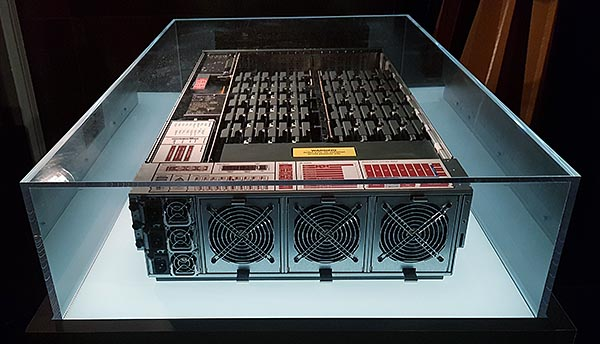
\includegraphics[width=10cm]{Kenenbek/images/yadro-tatlin.jpg}
\caption{Система хранения данных Татлин.}
\label{fig:yadro-tatlin}
\end{figure}

\par 
Платформа Tatlin представляет собой семейство систем хранения данных корпоративного уровня, предназначенных для решения широкого спектра задач и обладающих показателями производительности, плотности и стоимости владения. Основой архитектуры системы служит высокоскоростная отказоустойчивая фабрика PCI Express, которая в совокупности с технологией виртуализации SR-IOV обеспечивает рекордную производительность операций ввода-вывода. Схема компонент Татлина изображена на рис. ~\ref{fig:tatlin}.

\begin{figure}[!ht]
\centering
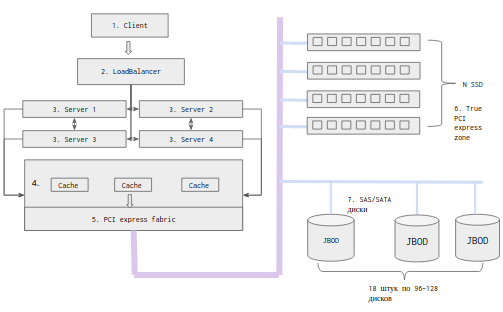
\includegraphics[width=10cm]{Kenenbek/images/tatlin.png}
\caption{Составные блоки системы Татлин.}
\label{fig:tatlin}
\end{figure}

\par 
С ростом объема дисков возникла потребность в новых способах обеспечения сохранности данных. В продуктах, созданных на базе платформы Tatlin, реализован собственный механизм обеспечения целостности данных, реализованный на базе избыточных кодов Рида-Соломона. Помимо высокой степени защиты, гибких политик избыточности и возможности использования гетерогенных носителей система обладает большей надежностью за счет уменьшения времени на восстановление в случае выхода дисков из строя. Наличие когерентного дублированного энергонезависимого (NRVAM) кэша на запись добавляет производительности и отказоустойчивости. Расширяемая до объема 2 Тбайт кэш-память с временем задержки менее 200 нс обеспечивает режим Active-Active для всех контроллеров системы хранения данных, а также реализует аппаратное ускорение обработки данных при помощи микроконтроллера на базе архитектуры MIPS64. 



В настоящее время в наличии имеется следующая конфигурация системы хранения данных (рис. \ref{fig:tatlin-setup}).

\begin{figure}[H]
\centering
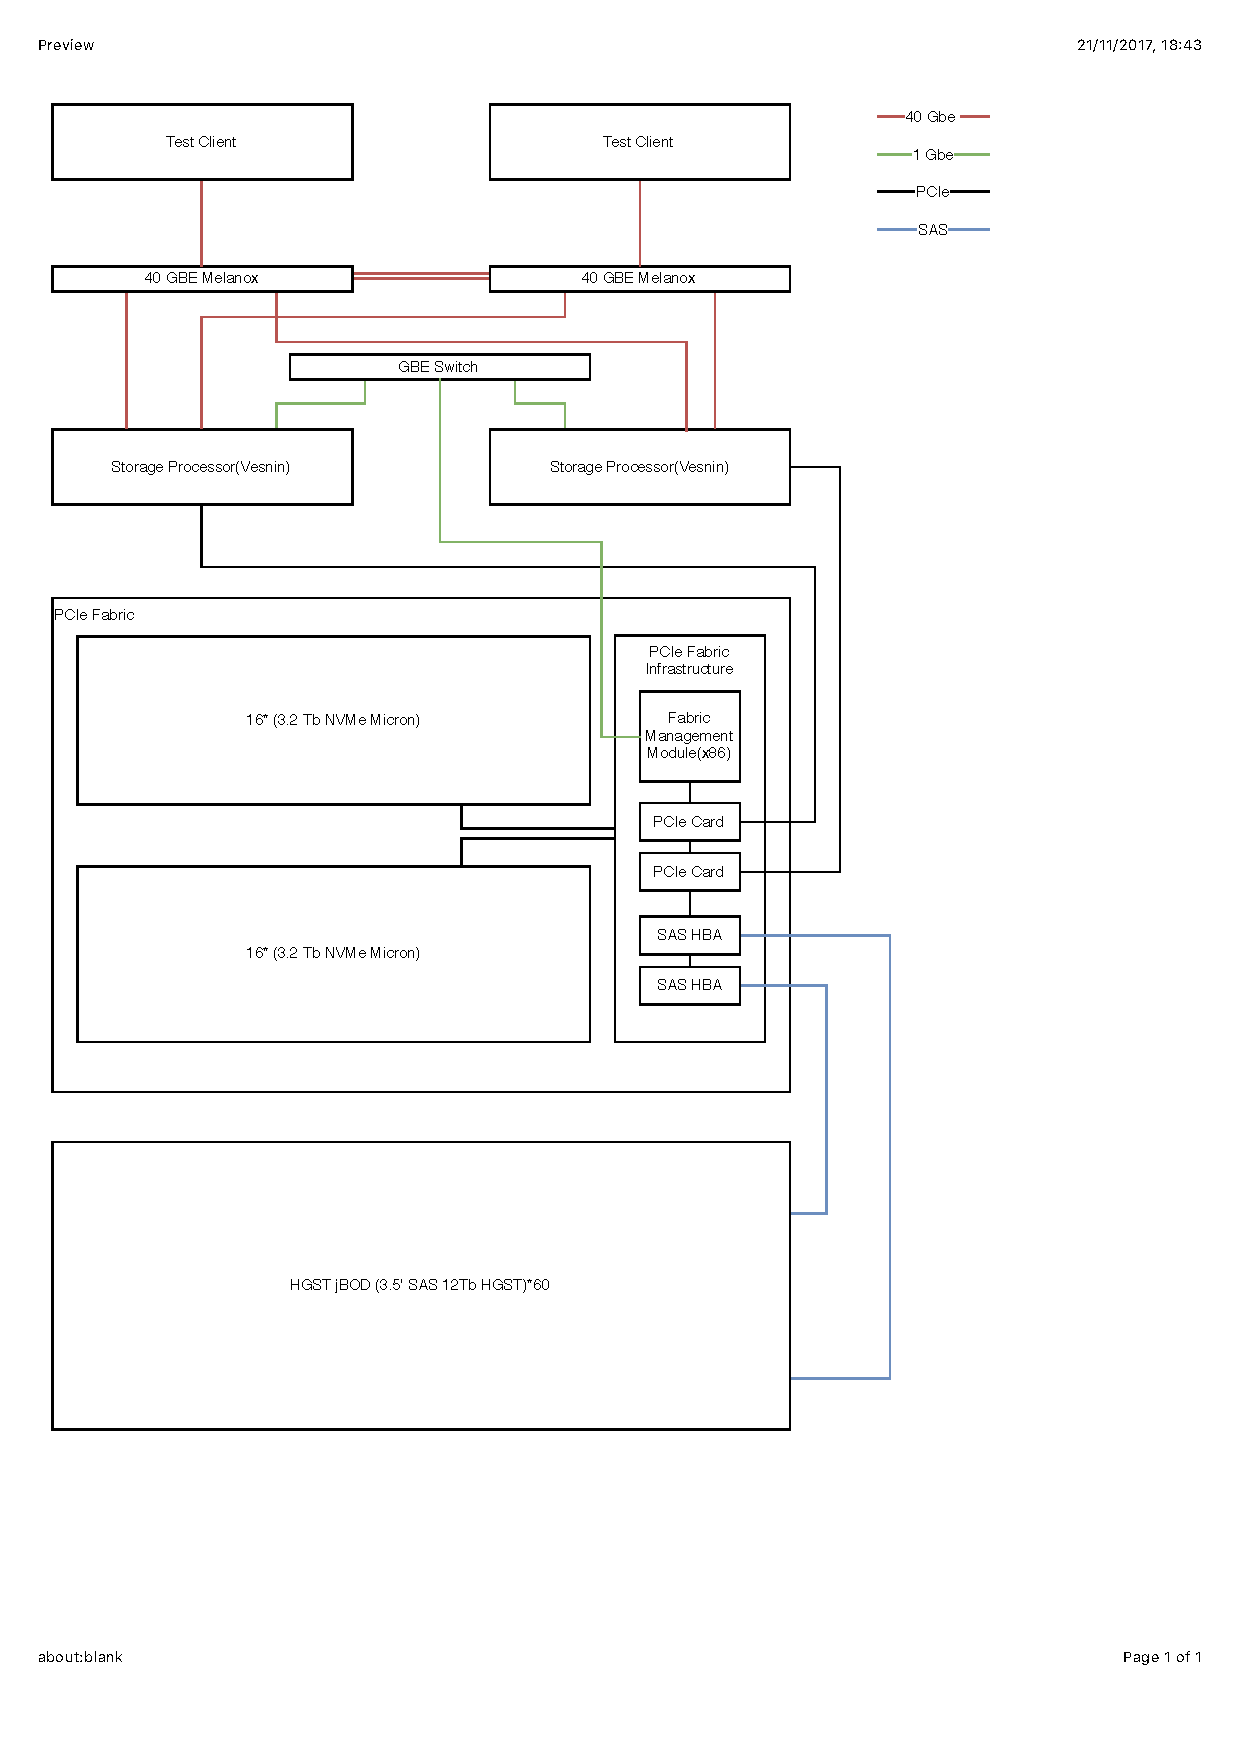
\includegraphics[width=10cm]{Kenenbek/images/tatlin-setup.pdf}
\caption{Тестовая конфигурация СХД Татлин}
\label{fig:tatlin-setup}
\end{figure}

Описание компонент приведено в таблице:

\begin{table}[]
\centering
\caption{Компоненты СХД Татлин}
\label{tab:tatlib-setup}
\begin{tabularx}{\textwidth}{|X|X|X|}
\hline
Наименование      & Кол-во  & Функциональность компонента                                                                                                                                                                                                                                    \\ \hline
Client            & 1-неогр & Устройство, которое создаёт нагрузку на СХД Татлин в виде создания запросов на запись/чтение файлов.                                                                                                                                                           \\ \hline
Storage Processor & 1-4     & Электронный блок, интегральная схема (микропроцессор), исполняющая машинные инструкции (код программ), главная часть аппаратного обеспечения компьютера или программируемого логического контроллера. Иногда называют микропроцессором или просто процессором. \\ \hline
GBE Switch        & 1       & Коммутатор внутренней сети управления.                                                                                                                                                                                                                         \\ \hline
GBE Melanox       & 1       & Сетевой адаптер -- устройство, позволяющее компьютеру взаимодействовать с другими устройствами сети (клиентом).                                                                                                                                                \\ \hline
PCIe Fabric       & 1       & Управление кэшем. Возмножность энергонезависимо управлять, читать, записывать данные на конечные дисковые накопители.                                                                                                                                          \\ \hline
PCIe Card         & 1-2     & Сетевой адаптер -- дополнительное устройство, позволяющее компьютеру взаимодействовать с другими устройствами сети (GBE Card).                                                                                                                                 \\ \hline
SAS HBA           & 1-2     & Сетевой адаптер -- устройство, позволяющее компьютеру взаимодействовать с другими устройствами сети (клиентом).                                                                                                                                                \\ \hline
HGST JBOD         & 1-2     & Сетевой адаптер -- устройство, позволяющее компьютеру взаимодействовать с другими устройствами сети (клиентом).                                                                                                                                                \\ \hline
\end{tabularx}
\end{table}


Для моделирования СХД Татлин на основании рис. \ref{fig:tatlin-setup} были реализованы функции, как показано на рис.  ~\ref{fig:norm-tatlin}:

\begin{itemize}
\item ClientExecutor (Клиент) 
\item LoadBalancer (БН)
\item ServerExecutor (Контроллер (Веснин))
\item PCIeFabric (PCIe фабрика)
\begin{itemize}
\item CacheExecutorRead
\item CacheExecutorWrite
\end{itemize}
\item DiskExecutor (Диск)
\end{itemize}

Стоит отметить, что сетевые адаптеры включены в состав смежных с ними компонент СХД.

\begin{figure}[!ht]
\centering
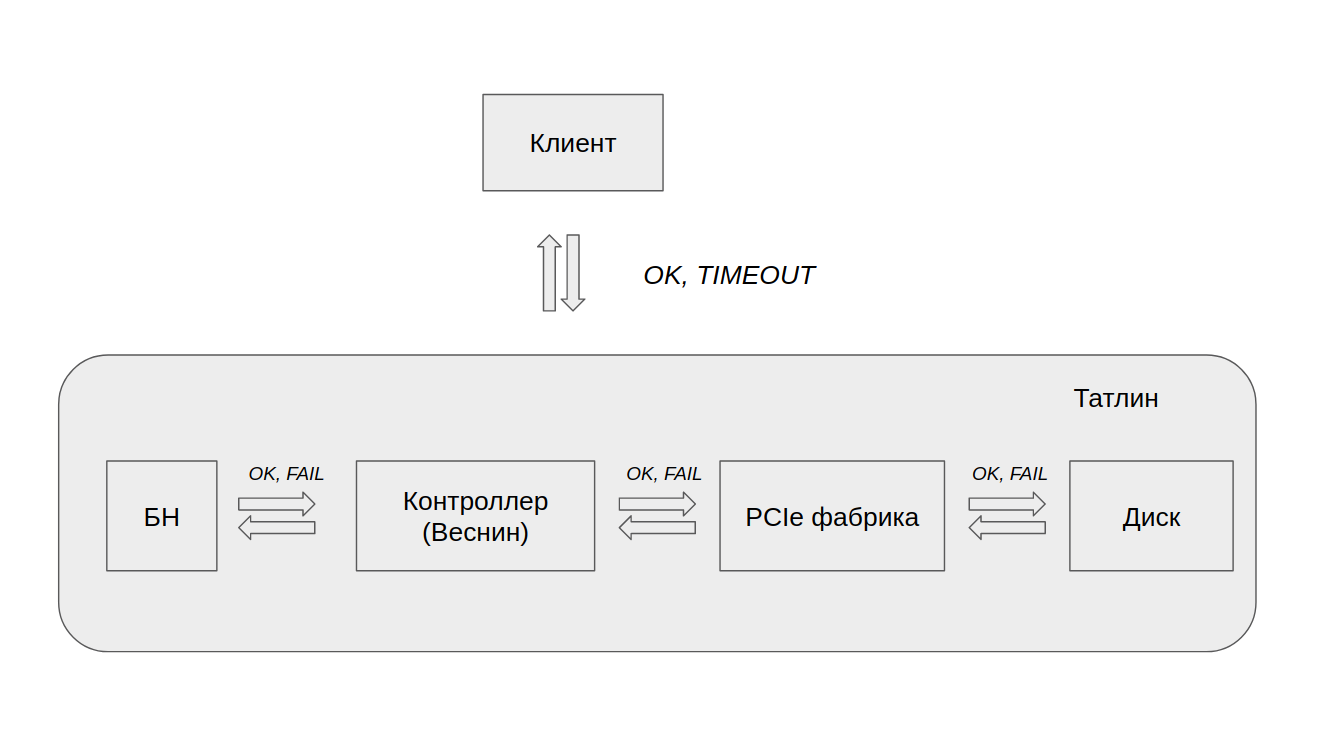
\includegraphics[width=10cm]{Kenenbek/images/norm.png}
\caption{Нормальный режим работы СХД Татлин. БН -- балансировщик нагрузки}
\label{fig:norm-tatlin}
\end{figure}

\par 
Балансировщик нагрузки (БН) при обращении клиента создаёт три соответсвующих процесса: один процесс отвечающий за логику серверной части, второй -- за PCIe фабрику и третий -- за конечный дисковый носитель. Описание каждого из них дано в последующих главах.

\par 

В конечном итоге мы получаем следующую схему, как показано на рис. ~\ref{fig:simtatlin}.
\begin{figure}[!ht]
\centering
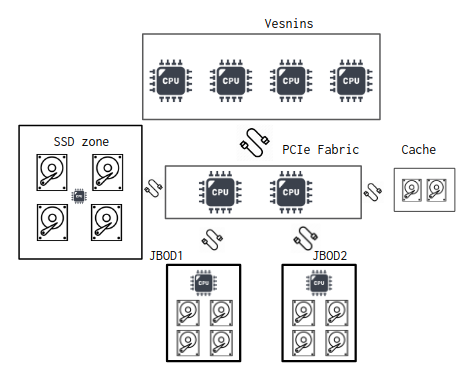
\includegraphics[width=\textwidth]{Kenenbek/images/t-scheme.png}
\caption{Система Татлин, выраженная в блоках симуляции}
\label{fig:simtatlin}
\end{figure}


\subsection{Описание Клиента}
\par 
Модель клиент-сервер представляет собой распределенную структуру приложения, которая разделяет задачи или рабочие нагрузки между поставщиками ресурса или службы, называемыми серверами и запросами обслуживания, называемыми клиентами. Часто клиенты и серверы общаются по компьютерной сети на отдельном оборудовании, но как клиент, так и сервер могут находиться в одной и той же системе. Хост сервера запускает одну или несколько серверных программ, которые делят свои ресурсы с клиентами. Клиент не использует ни один из своих ресурсов, но запрашивает содержимое или функцию обслуживания сервера. Поэтому клиенты инициируют сеансы связи с серверами, которые ждут входящих запросов. Схема изображена на рис. ~\ref{fig:client}.

\begin{figure}[!ht]
\centering
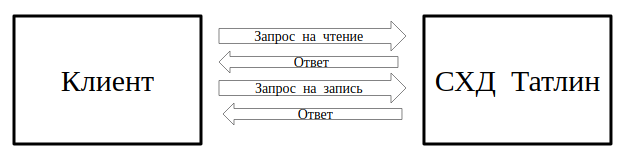
\includegraphics[width=10cm]{Kenenbek/images/client.png}
\caption{Взаимодействие клиент-сервер.}
\label{fig:client}
\end{figure}

\par 
В текущий момент времени клиентская часть реализует следующую последовательность действий:

\begin{enumerate}
\item\label{itm:client-a} Обращение к БН для того, чтобы узнать имя сервера, который будет обслуживать действующий запрос. 
\item Инициализировать соединение с сервером 

\item Цикл до тех пор пока не отправятся все пакеты:
	\begin{itemize}
		\item Отправка пакета данных 
			\begin{itemize}
				\item В случае аномалии вернуться к пункту \ref{itm:client-a}
			\end{itemize}
		\item Ожидание сообщения об успешной записи пакета на диск
			\begin{itemize}
				\item В случае аномалии вернуться к пункту \ref{itm:client-a}
			\end{itemize}
	\end{itemize}
\item Завершение соединения
\end{enumerate}



\subsection{Описание Балансировщика Нагрузки}
\par 
При проведении ресурсоёмких вычислений балансировка нагрузки улучшает распределение рабочих нагрузок на нескольких вычислительных ресурсах, таких как компьютеры, компьютерный кластер, сетевые ссылки, центральные процессоры или дисковые накопители. Балансировка нагрузки направлена на оптимизацию использования ресурсов, максимизацию пропускной способности, минимизацию времени отклика и предотвращение перегрузки любого отдельного ресурса. Использование нескольких компонентов с балансировкой нагрузки вместо одного компонента может повысить надежность и доступность благодаря избыточности. Балансировка нагрузки обычно включает специализированное программное обеспечение или аппаратное обеспечение, такое как многоуровневый коммутатор.
\par
Данный процесс завершит свою деятельность после завершения других процессов, которые симулируют работу система Татлин. В текущий момент времени Балансировщик Нагрузки реализует следующую последовательность действий: 

\begin{itemize}

\item Бесконечный цикл:
	\begin{itemize}
		\item Ожидание запроса на соединение от клиента
		\item Установление соединения
		\item Выбор контроллера, который будет обслуживать запросы от клиента
		\item  Завершение соединения
	\end{itemize}
\end{itemize}

\subsection{Описание Серверной части}
\par 
При вычислении сервер представляет собой компьютерную программу или устройство, которое обеспечивает функциональность для других программ или устройств, называемых «клиентами». Эта архитектура называется клиент-серверной моделью. Вычисления распределяются между несколькими процессами или устройствами. Один сервер может обслуживать несколько клиентов, а один клиент может использовать несколько серверов. Клиентский процесс может работать на одном устройстве или может подключаться по сети к серверу на другом устройстве.

\begin{figure}[!ht]
\centering
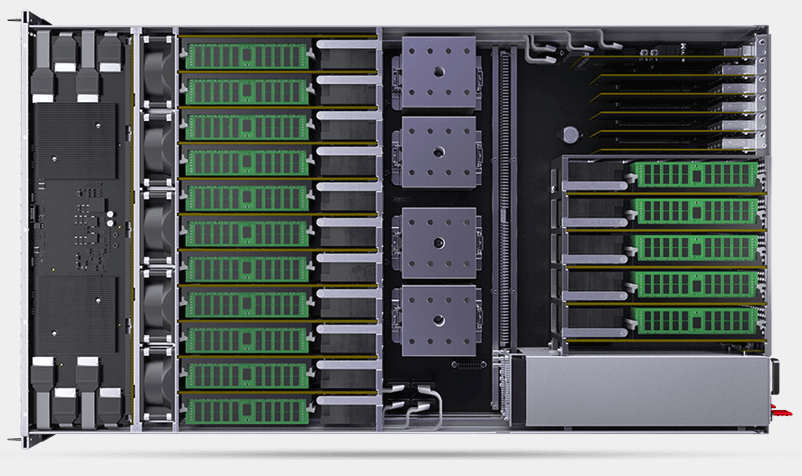
\includegraphics[width=10cm]{Kenenbek/images/vesninproc.png}
\caption{Процессор Веснин.}
\label{fig:vesninproc}
\end{figure}

\par 
В сервер Веснин, устанавливаемый в СХД Татлин, можно поставить до 4 процессоров (соответственно до 48 ядер POWER8) и количество памяти до 8 ТБ. Дисковая подсистема сервера может включать до 24 дисков стандарта NVMe. Диски равномерно распределены по четырём процессорам с помощью двух PCI Express свитчей PMC 8535. Каждый свитч логически разделен на три виртуальных свитча: один x16 и два x8. Таким образом, на каждый процессор доступно PCIe x16, или до 16 ГБ/с. К каждому процессору подключено по 6 NVMe дисков. Суммарно, мы ожидаем пропускную способность до 60 ГБ/с со всех дисков.
\par
Сервер реализует следующую последовательность действий: 

\begin{itemize}
\item Установка соединения с клиентом
\item Бесконечный цикл:
	\begin{itemize}
		\item Ожидание пакета от клиента
		\begin{itemize}
			\item Если произошла аномалия, то выйти из цикла
		\end{itemize}
		
		\item Отправка пакета PCIe фабрике
		\begin{itemize}
			\item Если произошла аномалия, то выйти из цикла
		\end{itemize}		
		\item  Отправка клиенту сообщения об успешной записи пакета на диск 
		\begin{itemize}
			\item Если произошла аномалия, то выйти из цикла
		\end{itemize}
		\begin{itemize}
			\item Если пакет последний, то выйти из цикла
		\end{itemize}
	\end{itemize}
\end{itemize}

\subsection{Описание PCIe фабрики }

Технология ExpressFabric предназначена для замены «мостовых» и коммутационных устройств. Такая ситуация возможна, потому что практически все компоненты, составляющие основу центров обработки данных, процессоры, устройства хранения данных и устройства связи, имеют PCIe как по крайней мере одно из своих соединений. Используя PCIe в качестве основной передаточного узла, все компоненты могут взаимодействовать напрямую. Исключив необходимость перевода с PCIe (на компонент) на Ethernet или InfiniBand (в качестве двух общих альтернатив), стоимость и мощность стойки могут быть существенно уменьшены. Кроме того, связь между компонентами также снижает задержку сети.

Фабрика реализует следующую последовательность действий: 

\begin{itemize}
\item Установка соединения с сервером
\item Бесконечный цикл:
	\begin{itemize}
		\item Ожидание пакета от сервера
		\begin{itemize}
			\item Если произошла аномалия, то выйти из цикла
		\end{itemize}
		
		\item Отправка пакета на запись в кэш
		\item Отправка пакета на запись на диск		
		\item  Отправка серверу сообщения об успешной записи пакета на диск 
		\begin{itemize}
			\item Если произошла аномалия, то выйти из цикла
		\end{itemize}
		\begin{itemize}
			\item Если пакет последний, то выйти из цикла
		\end{itemize}
	\end{itemize}
\end{itemize}

\subsection{Описание Конечного дискового носителя}
\par 
Жесткий диск, жесткий диск или жесткий диск - это устройство электромеханического хранения данных, которое использует магнитное хранилище для хранения и извлечения цифровой информации с использованием одного или нескольких жестких быстро вращающихся дисков (пластин), покрытых магнитным материалом. Шпиндели соединены с магнитными головками, обычно расположенными на движущемся рычаге привода, которые считывают и записывают данные на поверхности пластин. Доступ к данным осуществляется произвольным образом, что означает, что отдельные блоки данных могут быть сохранены или извлечены в любом порядке и не только последовательно. Жесткие диски являются типом энергонезависимого хранилища, сохраняя сохраненные данные даже при выключенном питании.
\par 
Современный жесткий диск записывает данные, намагничивая тонкую пленку ферромагнитного материала на диске. Последовательные изменения направления намагничивания представляют двоичные биты данных. Данные считываются с диска путем обнаружения переходов при намагничивании. Пользовательские данные кодируются с использованием схемы кодирования, которая определяет, как данные представлены магнитными переходами.
\par 
Конечный дисковый носитель реализует следующую последовательность действий.

\begin{itemize}
\item Установка соединения с PCIe фабрикой
\item Бесконечный цикл:
	\begin{itemize}
		\item Ожидание пакета от сервера
		\begin{itemize}
			\item Если произошла аномалия, то выйти из цикла
		\end{itemize}
		
		\item Отправка пакета на запись в кэш
		\item Отправка пакета на запись на диск		
		\item  Отправка серверу сообщения об успешной записи пакета на диск 
		\begin{itemize}
			\item Если произошла аномалия, то выйти из цикла
		\end{itemize}
		\begin{itemize}
			\item Если пакет последний, то выйти из цикла
		\end{itemize}
	\end{itemize}
\end{itemize}

\subsection{Аномалии в СХД Татлин}
На данный в дискретно-событийной библиотеке реалиазовано два вида аномалий: серверов и сетей, что и нашло отражение при симулировании СХД Татлин.

Сценарий развития аномалии:

\begin{itemize}
\item Полностью выходит из строя один из серверов 
\item По получении сообщения о выхода из строя сервера, либо по таймауту по цепочке выходят из строя следующие процессы, обслуживающие передачу конкретного файла:
	\begin{itemize}
		\item  Клиент
		\item Балансировщик нагрузки
		\item PCIe фабрика
		\item Диск
	\end{itemize}
\end{itemize}

Схематическое представление выхода из строя сервера показано на рис. ~\ref{fig:bad-tatlin}.

\begin{figure}[!ht]
\centering
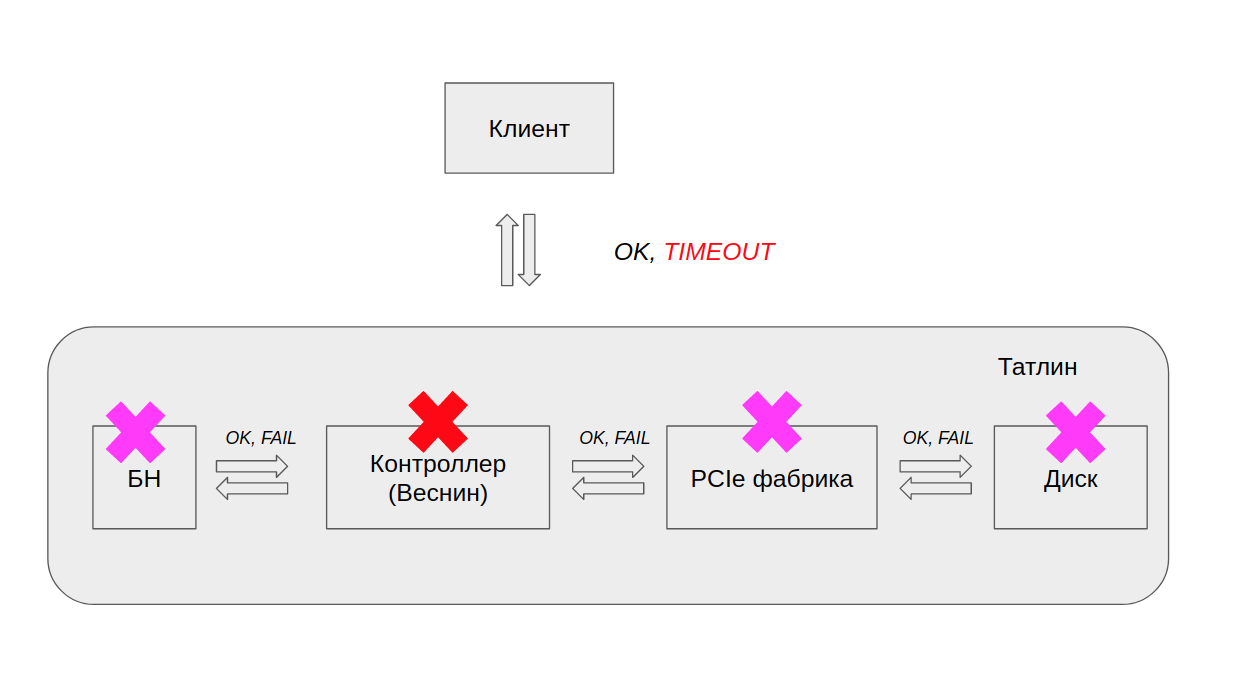
\includegraphics[width=10cm]{Kenenbek/images/bad.png}
\caption{Возникновение аномалии в СХД Татлин}
\label{fig:bad-tatlin}
\end{figure}

\subsection{Параметры запуска тестового прогона}

Начальные параметры компонент СХД Татлин заданы в файле $platform.xml$. Параметры дисковых контроллеров, сетей, конечных дисковых носителей и отображены в таблицах ~\ref{tab:storage-contollers}, ~\ref{tab:links} и ~\ref{tab:storage} соответственно:

\begin{table}[]
\centering
\caption{Параметры дисковых котроллеров}
\label{tab:storage-contollers}
\begin{tabularx}{\textwidth}{|l|l|l|} 
\hline
                     & Имя       & Скорость, Гфс  \\ 
\hline
Storage controller 1 & Server 1~ & 1              \\ 
\hline
Storage controller 2 & Server 2~ & 1              \\ 
\hline
Storage controller 3 & Server 3~ & 1              \\ 
\hline
Storage controller 4 & Server 4~ & 1              \\
\hline
\end{tabularx}
\end{table}


\begin{table}
\centering
\caption{Параметры сетей}
\label{tab:links}
\begin{tabularx}{\textwidth}{|l|l|l|} 
\hline
Имя сети               & Скорость, ГБ/с & Задержка сети, нс  \\ 
\hline
Client\_Server1        & 10             & 5                  \\ 
\hline
Client\_Server2        & 10             & 5                  \\ 
\hline
Client\_Server3        & 10             & 5                  \\ 
\hline
Client\_Server4        & 10             & 5                  \\ 
\hline
Server1\_FabricManager & 12             & 5                  \\ 
\hline
Server2\_FabricManager & 12             & 5                  \\ 
\hline
Server3\_FabricManager & 12             & 5                  \\ 
\hline
Server4\_FabricManager & 12             & 5                  \\ 
\hline
FabricManager\_SSD     & 12             & 5                  \\ 
\hline
FabricManager\_JBOD1   & 2              & 5                  \\ 
\hline
FabricManager\_JBOD2   & 2              & 5                  \\
\hline
\end{tabularx}
\end{table}


\begin{table}[]
\centering
\caption{Параметры конечных дисковых носителей}
\label{tab:storage}
\begin{tabularx}{\textwidth}{|l|l|l|l|}
\hline
Идентификатор & Размер, ТБ & Скорость на чтение, ГБ/с & Скорость на запись, ГБ/с \\ \hline
JBOD1         & 100        & 1                        & 1                        \\ \hline
JBOD2         & 100        & 1                        & 1                        \\ \hline
SSD           & 50         & 10                       & 10                       \\ \hline
\end{tabularx}
\end{table}

\subsection{Валидация результатов}
\par 
Проверка и валидация компьютерных имитационных моделей проводится при разработке имитационной модели с конечной целью создания точной и достоверной модели. Моделирование все чаще используется для решения проблем и содействия принятию решений. Т.к симуляция -- это приблизительная имитация систем реального мира, и она никогда точно не имитируют реальную систему. В связи с этим модель должна быть проверена и точность её подтверждена до степени, необходимой для применения модели в реальном мире.

\par Одним из преимуществ симулятора является то, что он способен выдавать результаты в формате реального стенда. Для проверки достоверности работы симулятора предлагается использовать следующую схему, показанную на рис. ~\ref{fig:probtatlin}. Probtatlin -- дополнительный сервис, реализованный на языке программирования Python и используемый для настройки параметров симулятора. Проверка и валидация - это итеративный процесс, который происходит во время разработки модели.
\par Предлагается:
\begin{itemize}
\item Устроить прогон тестового стенда
\item Сохранить результаты выдачи транслятора в базу данных
\item Устроить прогонь симулятора и сохранить его
\item Сравнить результаты. В случае, если желаемая достоверность достигнута, закончить.
\item В случае, если результаты разнятся, запустить сервис Probtatlin для настройки параметров симулятора.
\item Повторять процесс до тех пока результат не сойдётся.

\end{itemize}


\begin{figure}[!ht]
\centering
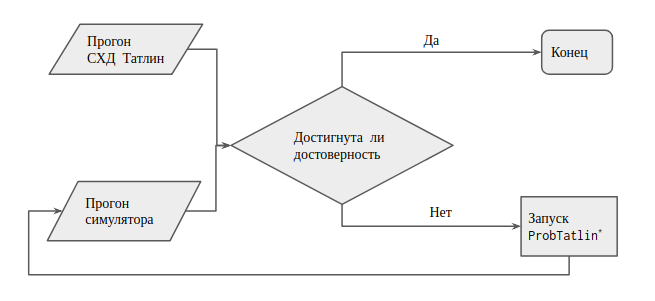
\includegraphics[width=\textwidth]{Kenenbek/images/probtatlin.png}
\caption{Cхема валидации результатов симулятора.}
\label{fig:probtatlin}
\end{figure}

\par 

